
% Introduce the NOvA experiment
%Introduce the NOvA detectors and give big picture overview
The NuMI Off-axis $\nu_e$ Appearance (NOvA) experiment 
is designed to make precise measurements of muon neutrino
disappearance and electron neutrino appearance in a muon neutrino
beam.  
The experiment consists of two functionally equivalent
detectors which measure the neutrino energy and flavour composition of 
the Neutrinos at the Main Injector (NuMI) beam. 
The detectors are constructed from PVC tubes filled with liquid
scintillator and are highly granular to distinguish neutrino induced
signals and background.
The 300~ton near detector is located on site at Fermilab 1.015~km  
from the NuMI target. The 14~kiloton far detector is located at a site
near Ash River, Minnesota and is 810~km from the NuMI target. 
The baseline and mean neutrino energy are chosen such that the far
detector sees the first oscillation maximum driven by $\Delta
m_{32}^2$. 
Both detectors are placed off-axis from the centre
of the NuMI beam to enhance the sensitivity to electron neutrino
appearance and muon neutrino disappearance.
%by 14.6~mrads.

The original design of the NOvA experiment is laid out in the
technical design report (TDR) \cite{TDR} and the constructed experiment
design differs only slightly. The details
of the constructed experiment, including the neutrino beam source and
the two detectors, are discussed in the following chapter.


\section{The NuMI Beam}

The NOvA experiment's neutrino source is the Neutrinos at
the Main Injector (NuMI) beam at Fermilab. The following section
briefly describes the process by which the NuMI beam is
created. More details are available in Ref~\cite{NuMI}.

The NuMI beam-line extracts batches of approximately $4.8 \times
10^{13}$ 120~GeV protons from the Main
injector and directs them onto a 0.95~m long graphite
target. Each extraction of protons is known as a beam spill. There is
typically an interval of 1.33~s between beam spills.

An instructive diagram of the NuMI beam facility is presented in
Figure~\ref{fig:NuMI}, which shows the beam components including the 
Target Hall, Decay Pipe, Hadron Monitor, Absorber and Muon Monitors. 
Within the target hall, collisions between the accelerated protons and
the carbon atoms of the 
target produce a plethora of secondary particles (mostly pions and
kaons). The charged mesons of one sign (or the other) are focused into
a beam by two magnetic focussing horns. 
The resulting beam of charged mesons then enters the 675~m long He
filled Decay Pipe. Along this length the 
mesons decay predominantly to charged leptons and neutrinos. 
The decay pipe is followed by the Hadron Monitor, the Absorber, Muon
Monitors and about 240~m of rock. 
The remaining
muons are absorbed by the rock leaving a beam of
neutrinos. After the rock the beam 
arrives at the NOvA near detector before continuing through the
Earth's crust for 810~km where it reaches the NOvA far detector.

% The Main Injector accepts 12 batches, each spanning a spill window of
% 10~$\mu$sec, of protons at a time. Each proton is accelerated up to
% 120~GeV and directed to 
% %A 10~$\mus$ pulse of 120~GeV protons, known as a beam spill, is
% %directed to
% collide with the 95~cm long NuMI graphite target. 
% There is typically an interval of 1.33~s between each beam spill. 

% NuMI beam figure
\begin{figure}
  \centering
  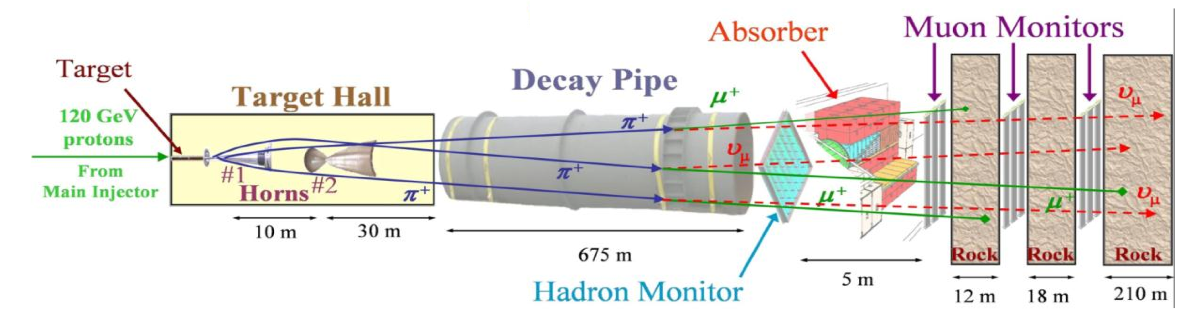
\includegraphics[width=1\textwidth]{../../img/beam/beam_diagram.png} 
  \caption{A diagram showing the layout of the NuMI beam. \cite{NuMI}}
  \label{fig:NuMI}
\end{figure}

\subsection{Focussing Horns}

Two magnetic horns are used to focus the mesons created 
by collisions of protons with the NuMI target into a
beam. Figure~\ref{fig:horn} shows the NuMI target, Horn~1, Horn~2 and
example meson trajectories. 
The design of the focussing horns allows three potential seperations
between 
Horn~1 and Horn~2 corresponding to a low, medium and high
energy beam. 
In the medium energy tune the Target is placed 1.3~m upstream from the
opening of Horn~1 while 
Horn~2 is placed 23~m downstream relative to the front face of Horn~1.
The NuMI horns are setup in the medium energy configuration
for the NOvA era.

The horns act as a lens where the focal
length is proportional to the momentum of the mesons.
Changing the current
direction within the focussing horns, choosing either forward or
reverse horn current, changes the direction of
the magnetic field and therefore the sign
of the mesons that are focussed. Operating the horns with forward or
reverse horn current selects positively or negatively charged mesons
respectively, leading to a predominantly neutrino or antineutrino beam
respectively. 

\begin{figure}
  \centering
  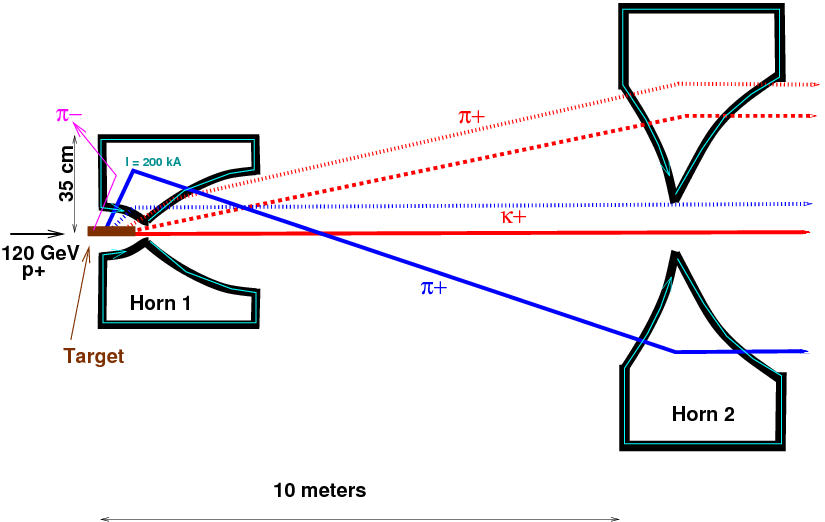
\includegraphics[width=0.8\textwidth]{../../img/beam/images_pion_tracks_in_horn.png}  
  \caption{
    A diagram of the magnetic focussing horns operating in forward
    horn current 
    mode. Positively charged mesons arriving from different directions
    are focussed by the combination of the two horns. The trajectory of
    positively charged mesons that are over or under focussed by Horn
    1 can be corrected by Horn 2. \cite{NuMI}
  }
  \label{fig:horn}
\end{figure}


\subsection{Off-axis Experiment Design}

The NOvA detectors are both placed 14~mrads off the axis of the NuMI
beam.
The dominant decay process used to produce a neutrino beam is a
two-body decay, where a
pion (or kaon) decays to a neutrino and a muon. The two body decay 
occurs isotropically in the parent particle's rest frame. 
In the lab frame the parent particle is not at rest when decaying, for
pion and kaon decay this boosts the neutrinos in the
direction of the parent particle.
For small angles, the flux per decay ($\Phi$) and energy ($E_\nu$) of
neutrinos produced by pion decay ($\pi \rightarrow \nu_{\mu} + \mu$)
are given by 

\begin{equation}
\Phi = \left( \dfrac{2\gamma}{1+\gamma^2 \theta^2} \right)^2 \dfrac{A}{4\pi z^2},
\label{eqn:NuPiFlux}
\end{equation}

\begin{equation}
E_{\nu} = \dfrac{0.43E_{\pi}}{1+\gamma^2\theta^2},
\label{eqn:NuPiEnrgy}
\end{equation}

\noindent where $E_{\pi}$ is the energy of the parent pion, $m_{\pi}$
the mass of the parent pion, $\gamma = E_{\pi}/m_{\pi}$, $\theta$ the
angle between the parent pion and outgoing
neutrino directions, A is the cross-sectional area and z is the distance
from the pion decay vertex.


Equations~\ref{eqn:NuPiFlux}~and~\ref{eqn:NuPiEnrgy} are shown as 
functions of pion energy for the Medium Energy NuMI Tune in
Figure~\ref{fig:NuPiFlux}. The Figure also shows the effect of four
off-axis angles ($\theta = 21~\text{mrads}$, $\theta =
14~\text{mrads}$, $\theta = 7~\text{mrads}$ and $\theta =
0~\text{mrads}$). 


Figure~\ref{fig:NuESpectra_MEAndLE} shows the number of neutrino
events as a function of the
charged current $\nu_{\mu}$ energy for the Low
(Figure~\ref{fig:NuESpectra_MEAndLE_a}) and 
Medium (Figure~\ref{fig:NuESpectra_MEAndLE_b}) Energy Tune for various
off-axis angles. The plots show that as the off-axis angle is
increased the mean and width of the energy distribution decreases.


For the Medium Energy Tune, figure~\ref{fig:NuPiFluxb} shows that at
14~mrad the neutrino energy
does not have a strong dependence on the parent pion energy.
In addition, figure~\ref{fig:NuESpectra_MEAndLE_b} shows that at
14~mrad the Medium
Energy Tune produces a narrow energy neutrino beam with approximately
4 times more neutrinos at 2~GeV than the on-axis scenario. This peak at
2~GeV is well matched to the expected energy of the first oscillation
maximum which is expected to occur at 1.6~GeV for
NOvA's L/E (experiment baseline to mean neutrino energy ratio) and for
$\Delta \textrm{m}_{32}^2=2.4~\textrm{meV}^2$. 

As described above, placing the detector off-axis increases the flux
at the expected oscillation maximum. In addition, the narrow energy
range of the off-axis beam reduces background
events. Neutral current events are an important background source
whose topologies can be hard to distinguish from electron showers
produced by $\nu_e$ charged current events. For neutral current events, the neutrino carries a
significant amount of the energy away and the energy visible within
the detector tends to
``feed down'' to lower energies. For a narrow band off-axis beam, this
feed down tends to shift the neutral current events towards lower energies
outside the $\nu_e$ appearance signal energy
window. Figure~\ref{fig:NuMIBeamComp} 
shows the number of $\nu_{\mu}$, $\nu_e$ and neutral current events as a function
of visible energy. The bulk of the neutral current events (black histogram) are
shown to shift below the signal region (red-hatched histogram).

The combination of reducing beam backgrounds and increasing the
neutrino flux at the oscillation maximum means that placing the
NOvA detectors at the off-axis angle of 14~mrads enhances the
sensitivity to oscillations driven by $\Delta m^2_{23}$.

\begin{figure}
  \centering
  \begin{subfigure}[b]{0.45\textwidth}
  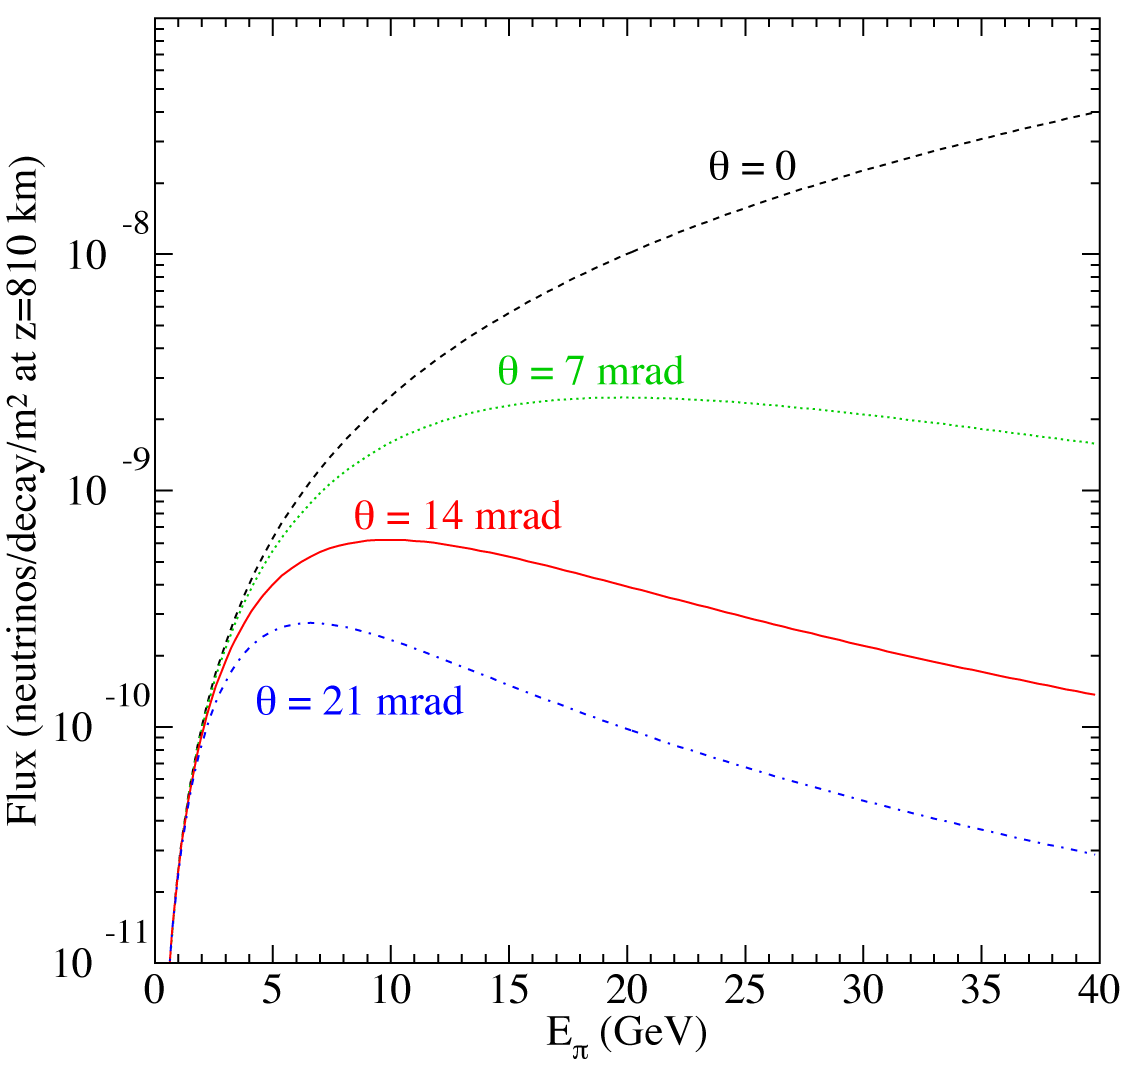
\includegraphics[width=\textwidth]{../../img/baird/beam/020-flux.png}
  \caption{Neutrino flux vs. pion energy. }
  \label{fig:NuPiFluxa}
  \end{subfigure}
  \hfill
  \begin{subfigure}[b]{0.45\textwidth}
  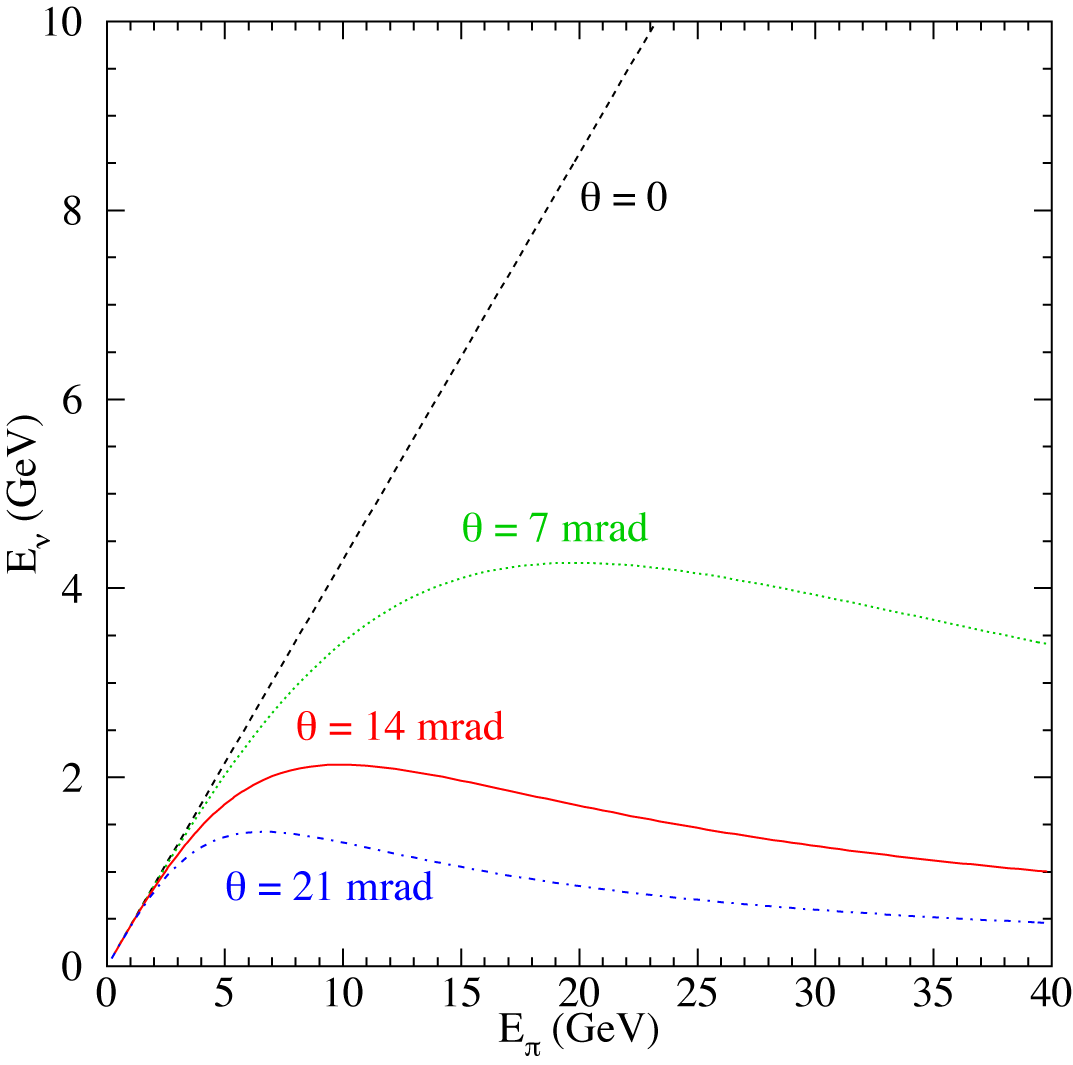
\includegraphics[width=\textwidth]{../../img/baird/beam/030-epi2enu.png}
  \caption{Neutrino vs. pion energy.}
  \label{fig:NuPiFluxb}
  \end{subfigure}
  \caption{The above distributions are for the medium energy tune NuMI
    beam as viewed from a site located
    800~km from the NuMI target and off-axis by an angle $\theta$. The
    left plot shows the neutrino flux as a function of the energy of
    the parent pion for different off-axis angles. The right plot
    shows the neutrino energy as a function of the parent pion energy
    for different off-axis angles.~\cite{TDR}}
  \label{fig:NuPiFlux}
\end{figure}



\begin{figure}
  \centering
  \begin{subfigure}[b]{0.45\textwidth}
    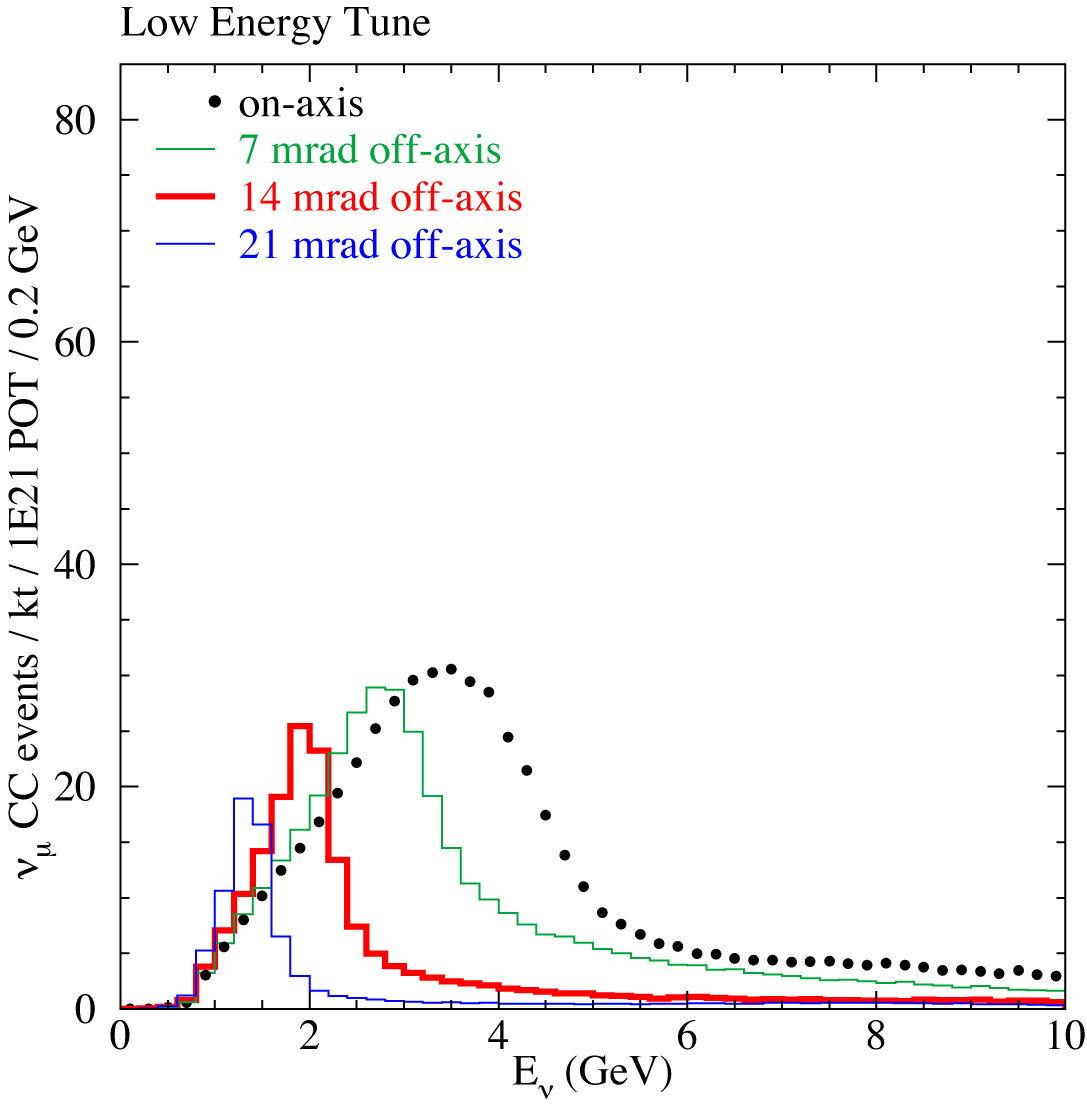
\includegraphics[width=\textwidth]{../../img/baird/beam/040-le-spectra.png}
    \caption{Low Energy Tune neutrino energy.  }
    \label{fig:NuESpectra_MEAndLE_a}
  \end{subfigure}
  \hfill
  \begin{subfigure}[b]{0.45\textwidth}
    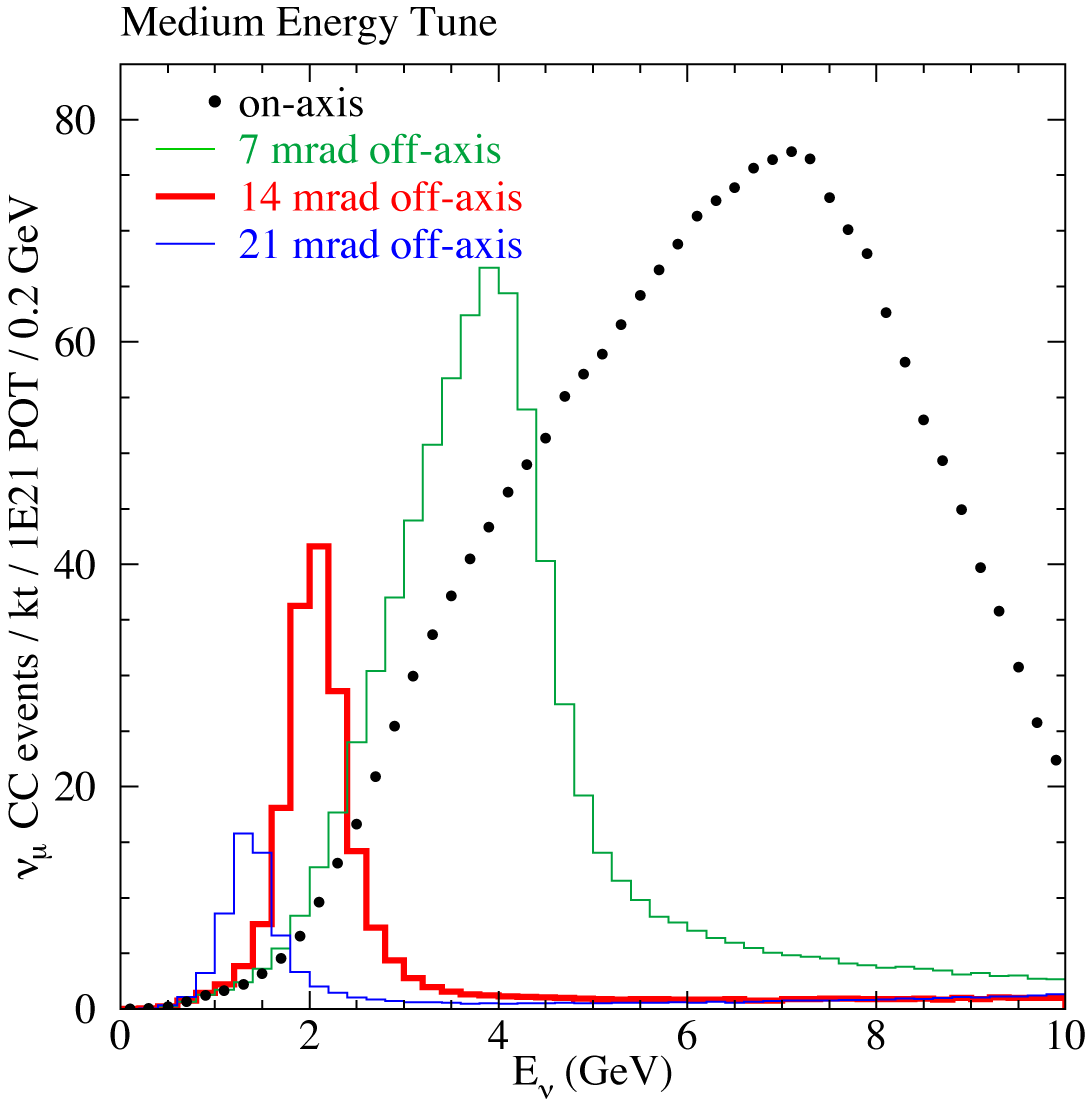
\includegraphics[width=\textwidth]{../../img/baird/beam/050-me-spectra.png}
    \caption{Medium Energy Tune neutrino energy.}
    \label{fig:NuESpectra_MEAndLE_b}
  \end{subfigure}
  \caption{Charged current $\nu_{\mu}$ event rates vs. neutrino
    energy in the absence of oscillations. The distributions are found
  for a detector which is 800~km from the NuMI target and for various
  off-axis angles.~\cite{TDR}}
  \label{fig:NuESpectra_MEAndLE}
\end{figure}


\begin{figure}
  \centering
  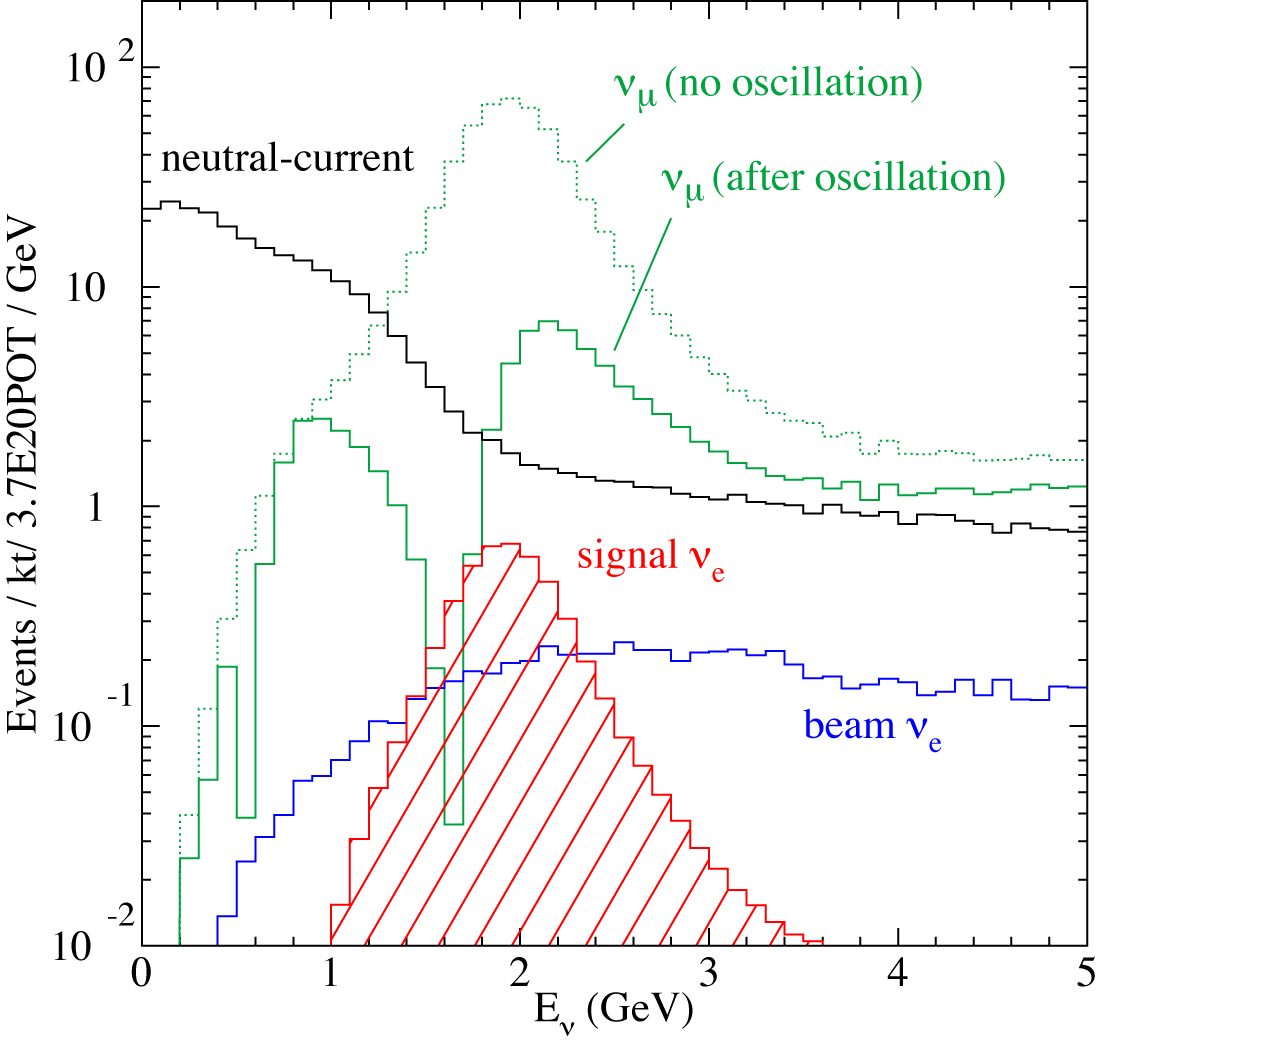
\includegraphics[width=0.5\textwidth]{../../img/beam/060-sig-and-bg-rates-thumb.png}
  \caption{Simulated visible energy distributions for $\nu_{\mu}$ charged current
    events with and without oscillations, $\nu_e$ oscillation signal events,
    intrinsic beam $\nu_e$ events and neutral current events. The
    simulation assumes an off-axis position of 12~km at 810~km, $\Delta m^2 = 2.5 \times 10^{-3}
    ~\textrm{eV}^2$, $\sin^2(2\theta_{23}) = 1.0$ and
  $\sin^2(2\theta_{13}) = 0.1$.~\cite{TDR}}
  \label{fig:NuMIBeamComp}
\end{figure}


\section{The NOvA Detectors}

% The NOvA experiment uses the NuMI beam, a near detector and a far
% detector to measure neutrino oscillation parameters. 
% The spectrum and composition of the NuMI beam is measured by both the
% near and far detectors. The near detector spectrum is extrapolated and
% compared with the far detector spectrum.

% The near detector is used to measure the un-oscillated
% neutrino energy spectrum and the electron neutrino component of the
% beam. The un-oscillated neutrino energy spectrum measured by the near
% detector is extrapolated to the far detector. The far detectors purpose is
% to measure the energy spectrum of the beam neutrinos for comparison
% with the extrapolated near detector energy spectrum.


The NOvA collaboration performs measurements of both $\nu_{\mu}$
disappearance and $\nu_e$ appearance and the NOvA detectors are
designed to be able to identify the muons and electrons produced in
charged-current neutrino interactions. 
The $\nu_e$ appearance
analysis has the potential to be overrun with neutral current
background events, 
a large source of background comes from $\pi^0$s produced in
neutral current 
events which can fake an electron shower.
The NOvA detectors are constructed from low Z materials (primarily
carbon) to aid in the distinction between neutrino interaction
signatures and the potentially troublesome background events.
The constructed detectors have a Moliere radius~\cite{pdg} of
approximately 11~cm which is equivalent to the depth (width) of two
(three) NOvA cells.  

%include all information common among both detectors.
A diagram of the two detectors
is shown in Figure~\ref{fig:bothDets}. 
The near and far NOvA detectors are almost functionally
identical. Besides
the different masses, there are a few physical
differences designed considering the proximity to the NuMI beam and
the depth of the detector relative to ground level. 
The smaller near detector has a so called ``muon catcher'' and
has a higher rate of readout. 
Whilst the far detector is constructed with an overburden to mitigate
the cosmic ray background.
The
construction common among both detectors will be discussed in the
following sub-sections. The details specific to the far and near detectors
will be discussed in sub-sections~\ref{sec:fardet} and
\ref{sec:neardet} respectively.

\begin{figure}
  \centering
  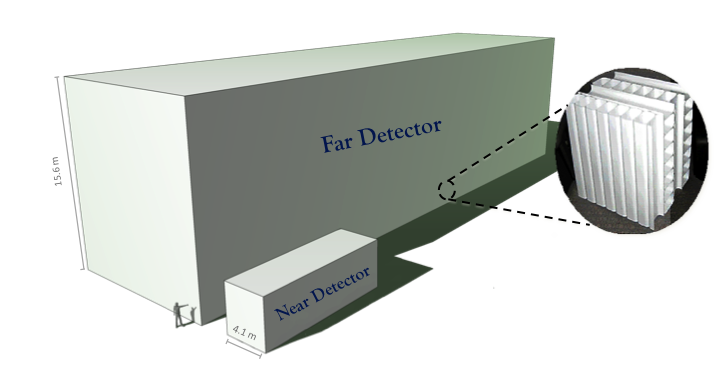
\includegraphics[width=0.8\textwidth]{../../img/det/gen/both_detectors.png} 
  \caption{
    Scaled depiction of the near and far NOvA
    detectors with respect to the average person.
    The alternating alignment of the NOvA
    cells is shown by the inset on the right hand side. }
  \label{fig:bothDets}
\end{figure} 


\subsection{The Basic NOvA Detector Element} \label{sec:cell}

The basic unit of the NOvA detectors is a rectangular rigid PVC
(Polyvinyl chloride) cell
which contains liquid scintillator and a wavelength-shifting
fibre. % An illustration of the NOvA cell is shown in
% Figure~\ref{fig:cell}. 
Figure~\ref{fig:cell} shows the NOvA cell, looped wavelength-shifting
fibre and an example charged particle.

The NOvA cells are made from highly reflective titanium dioxide loaded
rigid PVC. The cells have 2 to 4.5~mm thick walls, an interior depth
of 5.9~cm along the beam direction and an interior width of 3.8~cm
transverse to the beam direction. The thickness of the cell walls
varies due to structural considerations.
The length of the cells differs
between the two detectors, the far detector cells have a length of
15.5~m whilst the near detector cells are 3.6~m long.

The wavelength-shifting fibre, which is twice
the length of the 
cell, is looped at the bottom of the cell such that the captured light
travels in two directions to the instrumented top end of the cell. 
Both ends of the looped fibre are directed onto one pixel of an
Avalanche Photo Diode (APD) array.
The APD converts the light from the fibre into a digital signal.
% At
% the top end of the cell each end of the looped fibre is directed onto
% one pixel of an Avalanche Photo Diode (APD) array.




\subsection{Liquid Scintillator}

Approximately 65\% of the NOvA detector mass is composed of the liquid
scintillator held within the cells. The composition of the liquid
scintillator is detailed in Table~\ref{tab:scintComp}, which shows that
the scintillator is composed mainly of mineral oil along with 5.23\%
pseudocumene as the scintillant. The scintillant emits scintillation
light with a spectrum peaked between 360~-~390~nm. Wavelength shifting
chemical additives PPE and bis\_MSB are added to shift the initial
light spectrum to 400~-~450~nm to match the absorption spectra of the
wavelength-shifting fibre. 

% \begin{figure}
%   \centering
%   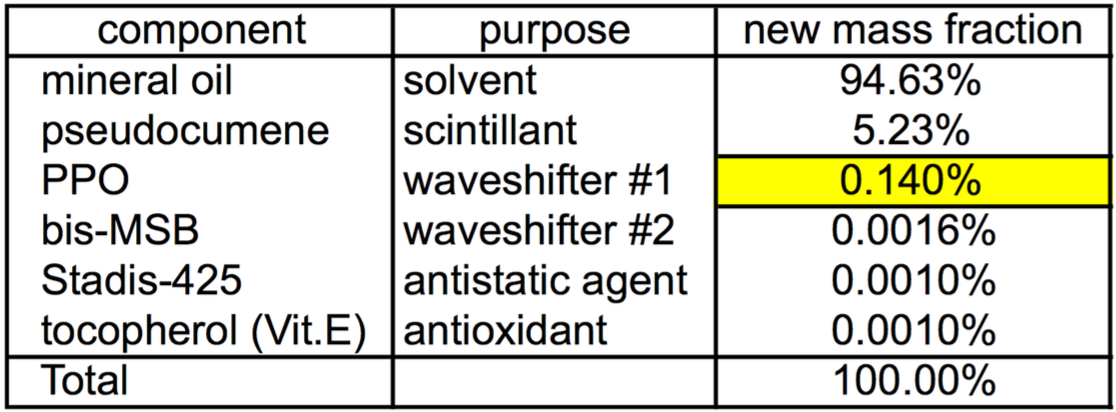
\includegraphics[width=0.8\textwidth]{../../img/det/gen/ScintCompTable.png}
%   \caption{Liquid scintillator composition. Table taken from \cite{scintillatorComp}. }
%   \label{fig:scintComp}
% \end{figure}

\begin{table}
  \centering
  %\begin{tabular}{| l | l | l |}
  \begin{tabular}{ l | l | l }
    %\hline
    Component & Purpose & Mass fraction \% \\ \hline
    mineral oil & solvent & 94.63 \\
    pseudocumene & scintillant & 5.23 \\
    PPO & waveshifter & 0.14 \\
    bis-MSB & waveshifter & 0.0016 \\
    stadis-425 & anti-static agent & 0.0010 \\
    tocopherol & antioxidant & 0.0010 \\
    %\hline
  \end{tabular}
  \caption{Chemical composition of the NOvA liquid scintillator. \cite{scintillatorComp} }
  \label{tab:scintComp}
\end{table}


\subsection{Wavelength Shifting Fibre}
The wavelength-shifting fibre has a diameter of 0.7~mm and a core of
polystyrene mixed with R27 dye (as the wavelength shifter) at a
concentration of 300~ppm. The fibre has two
coatings (contributing about 3\% of the fibre diameter) of materials
with a lower refractive index than the core
which facilitates total internal reflection within the fibre. The
fibre is first coated with a thin acrylic layer of PMMA and second
with fluor-acrylic. 

The 400~-~450~nm light emitted by the liquid scintillator is absorbed
by the fibre and then wavelength shifted to 490~-~550~nm. 
As light travels down the fibre it is attenuated, by a factor of about
10 in the far detector, with light in the range 520~-~550~nm
preferentially surviving. 


\subsection{Avalanche Photo Diode}

The light exiting the fibre ends is detected by an Avalanche
Photodiode (APD) and converted into an
electronic signal pulse. 
Figure~\ref{fig:apd} shows a photograph of a NOvA APD
containing an array
of 32 pixels. Each APD pixel is interfaced with both ends of a single
wavelength-shifting fibre. Each APD is connected to a front end board
that prepares the signals from the APD for the data acquisition
system. 

The NOvA APD was chosen because it has an 85\% quantum efficiency for
the 520~-~550~nm light exiting the fibre ends. 
The thermal noise generated by each APD is reduced by thermo-electric
coolers which cool the APDs to -15$^o$C. 


\begin{figure}
  \centering
  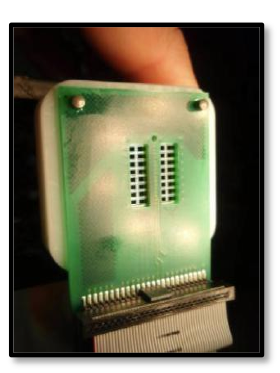
\includegraphics[width=0.4\textwidth]{../../img/det/gen/APD.png}
  \caption{The NOvA APD containing an array of 32 pixels.}
  \label{fig:apd}
\end{figure}





\subsection{Data Acquisition System}

%intro
NOvA's data acquisition system continuously reads out all
the information from the APDs. The information is temporarily stored
in a buffer farm and awaits a decision as to whether it should be
permanently recorded or rejected. The decision can be made by either
online triggering algorithms or by receiving a trigger signal from an
external source. The NuMI beam spill signal is an example of an
external source trigger.


%FEB
Each APD is continuously readout by an front end board, which handles the pedestal
subtraction and
pulse shaping for each signal from the APD. The pedestals are
determined for each APD pixel by measuring the baseline noise level.
The signal pulses are shaped with a characteristic rise and fall
time. When a signal is triggered the signal sample is read out along
with the three immediately preceding samples in a process called
``multi-point readout''. Once the data is permanently recorded, the
known pulse shaping 
parameters are used to fit the four samples and provide more
precise timing resolution. 

%FEB to DCM
The front end board transmits the digitised data to a data
concentrator module, which can take inputs from up to 64 front end
boards. 
%DCM to buffer node
Each data concentrator module collects all the information from the connected front end boards during a
50~$\mu s$ window (``microslice''). 
This data packet is then sent to and stored in the buffer farm
until online trigger processes decide whether to record or reject the
data. 


\subsection{Detector Assembly} \label{sec:detAssembly}

%build the detector starting with the cell:
The NOvA detectors are constructed from the cells described
in Section~\ref{sec:cell}. 16 cells are extruded together in one unit
to form an extrusion.
Figure~\ref{fig:extrusion} shows the end-on view of an extrusion with
a width of 63.5~cm and depth of 6.6~cm. 
Two extrusions are placed side by side to form an extrusion module
consisting of 32 cells.
Figure~\ref{fig:module} shows an extrusion module consisting of
32~cells, end plate, side seal, manifold cover, snout and
electronics box.
The
module ends are capped by the end plate so that the modules can
contain the liquid scintillator. The other end is capped by a manifold
cover which contains the liquid scintillator in the horizontal cells
and directs the 32 fibre end pairs to the 32 APD pixels in the NOvA
APD. 

Flat planes of cells are constructed from multiple modules glued
together side by side. 
Figure~\ref{fig:stackedPlanes} shows a cross-section of multiple plane
layers and the alternating orthogonal cell orientation.
The planes are layered with alternating orthogonal
orientations, such that the orientation of the cells making up the
plain alternate between horizontal and vertical from plane to
plane. The orthogonal 
orientation of the planes allows for three dimensional reconstruction
of tracks passing through multiple planes. Planes are glued together
in the orthogonal arrangement described above to form one solid
detector piece called a block, consisting of 32 or 24 planes in the
far detector or near detector respectively.


\begin{figure}
  \centering
  \begin{minipage}{.45\textwidth}
    \centering
    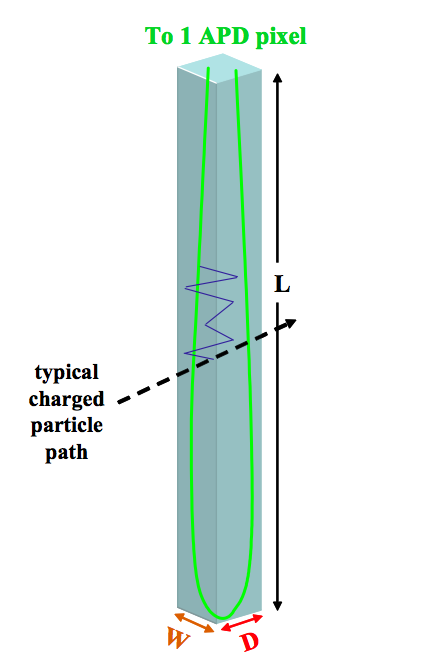
\includegraphics[height=0.4\textheight]{../../img/det/gen/nova_cell.png}
    \captionof{figure}{A NOvA cell consisting of an extruded
      PVC tube filled with liquid scintillator and a looped
      wavelength-shifting fibre. }
    \label{fig:cell}
  \end{minipage}%
  \hfill
  \begin{minipage}{.45\textwidth}
    \centering
    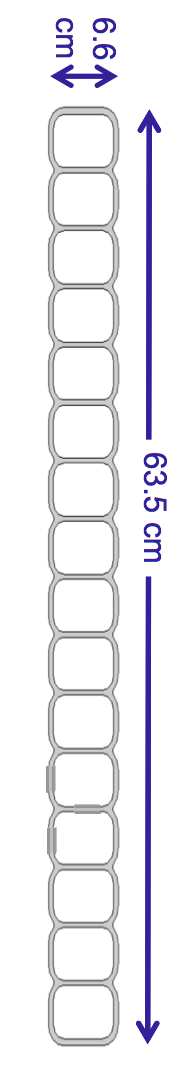
\includegraphics[height=0.4\textheight]{../../img/baird/det/extru_cross_section.png}
    \captionof{figure}{An end on view of an extrusion constructed from
      16 NOvA cells.\\}
    \label{fig:extrusion}
  \end{minipage}
\end{figure}




% %image of cell
% \begin{figure}
%   \centering
%   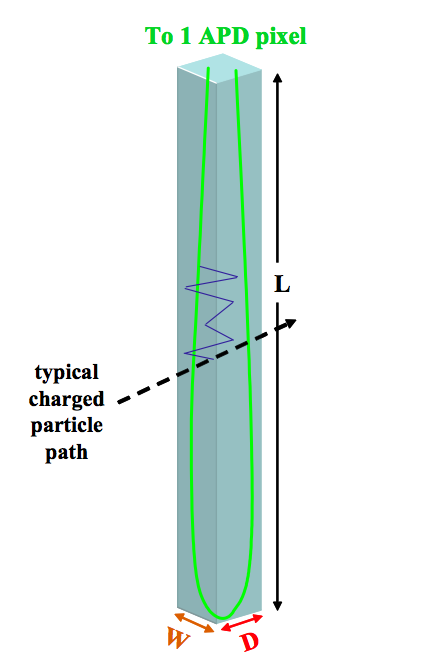
\includegraphics[width=0.5\textwidth]{../../img/det/gen/nova_cell.png}
%   \caption{A NOvA cell consisting of an extruded
%     PVC tube filled with liquid scintillator and a looped wavelength-shifting fibre.}
%   \label{fig:cell}
% \end{figure}

%  %extrusion
% \begin{figure}
%   \centering
%   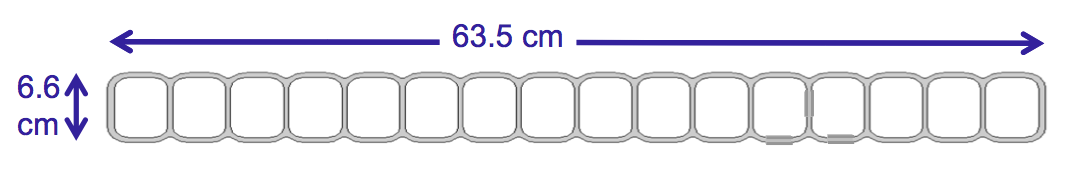
\includegraphics[width=0.5\textwidth]{../../img/det/gen/extru_cross_section.png}
%   \caption{A side on view of an extrusion constructed from16 cells.}
%   \label{fig:extrusion}
% \end{figure}

 %module
\begin{figure}
  \centering
  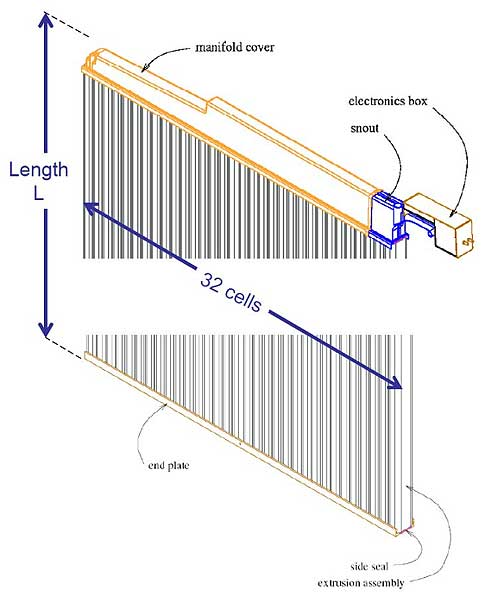
\includegraphics[width=0.5\textwidth]{../../img/det/gen/extrusionModule.jpg}
  \caption{A side on view of an extrusion module constructed from two
    extrusions of 16 cells, an end plate, a side seal, a manifold cover,
    a snout and an electronics box  }
  \label{fig:module}
\end{figure}

%orthogonally stacked planes
\begin{figure}
  \centering
  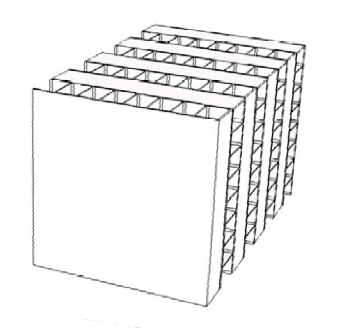
\includegraphics[width=0.5\textwidth]{../../img/det/gen/planes.png}
  \caption{Cut out of the NOvA detector showing the
    alternating orientation of the cells within the stacked planes.}
  \label{fig:stackedPlanes}
\end{figure}


\subsection{The Far Detector}\label{sec:fardet}

The 14~kiloton far detector is located 810~km from the NuMI target,
approximately 10~m below ground level and at an elevation of 372~m
above sea-level. The neutrino beam enters the
detector travelling at an angle of 3$^o$ upwards. The detector is
constructed, as described in Section~\ref{sec:detAssembly}, from
344,064 15.5~m long cells which form 896 planes normal to the beam
direction. The detector mass is approximately 65\% liquid scintillator
and 35\% PVC.

As described above, the far detector is built on the surface above sea
level so cosmic rays will be a major source of
background events. The background due to cosmic rays is mitigated
using selection cuts and a shielding overburden above the detector.
For the $\nu_{\mu}$ disappearance analysis the background is primarily
due to cosmic ray muons which are almost entirely removed using cuts. For
the $\nu_e$
appearance analysis, the background is primary cosmic ray photons
whose interactions within the detector can be mistaken for an electron
shower. 
During a six year run the far detector without overburden shielding will see
approximately 1600 background events due to cosmic ray photons. In
order to reduce this background source to less than one event requires
approximately 9 radiation lengths of material above the detector
surface. Additional radiation lengths will then help to contain any
showers caused by interactions within the overburden. With this in
mind, the far detector building was constructed with a 122~cm thick
concrete enclosure which supports a 15~cm thick overburden of
barite. Together, the concrete enclosure and barite overburden provide
12 radiation lengths of shielding.


\subsection{The Near Detector}\label{sec:neardet}

The NOvA near detector is located on site at Fermilab next to the
MINOS Hall. Figure~\ref{fig:cavern} is a diagram of the MINOS Hall
area showing the MINOS Shaft, NuMI beam-line, MINOS Hall, NuMI
Beam-line, 14.6~mrad off-axis beam and the NOvA Near Detector cavern. 
The near detector is 105~m
underground and 1.015~km from the NuMI target. The near detector
therefore sees a higher flux of NuMI neutrino events and a lower flux
of cosmic rays than the far detector.
The neutrino beam enters the detector travelling downwards at an angle
of 3$^o$. 

A diagram of the near detector is shown in
Figure~\ref{fig:neardet}. The Figure shows the NOvA Near Detector
cavern, access catwalks, and the fully active detector and muon catcher
detector sections.
The detector is constructed in a similar fashion to the far detector
with 20,192 cells arranged in 214 planes, each plane is comprised of 3
modules (except in the muon catcher). The detector has a width and
height (except in the muon catcher) of 4.2~m and a length of
15.8~m. The near detector is
functionally equivalent to the far detector with the exception of two
distinguishing features.

First, a muon catcher is placed at the downstream end of the near
detector in order to help range out muons
from few GeV charged current $\nu_{\mu}$ interactions which would not
otherwise stop within the detector.
The muon catcher is constructed from layers of steel and liquid
scintillator planes. The steel planes are 10~cm
thick and are separated by 
two (one horizontal and one vertically aligned) scintillator planes.
The vertical planes consist of
three modules while the horizontal planes are made from just two
modules. Therefore, the sets of steel and scintillator planes are
three modules wide (the same as the rest of the detector) but only
two modules high. Ten of these steel and
liquid scintillator plane sets are stacked to form the muon
catcher. The downstream end of the muon catcher has an additional 3
liquid scintillator planes.
% The muon catcher is added to the
% downstream end of the near detector in order to help range out muons
% from few GeV charged current $\nu_{\mu}$ interactions.

Second, the near detector electronics are setup to sample each channel
(APD pixel)
four times more frequently (every 125~ns) than in the far 
detector to help handle the data pileup. 
The near detector sees approximately 5-10 neutrino interactions per
beam spill (10 $\mu s$ window) while the far detector sees
approximately 60-70 cosmic rays per 550 $\mu s$ window spread out over
approximately 17 times more channels. The faster sampling rate
improves the timing resolution of hits in the detector. With better
timing resolution, pileup events are more easily distinguished from one
another. 




 %cavern diagram
\begin{figure}
  \centering
  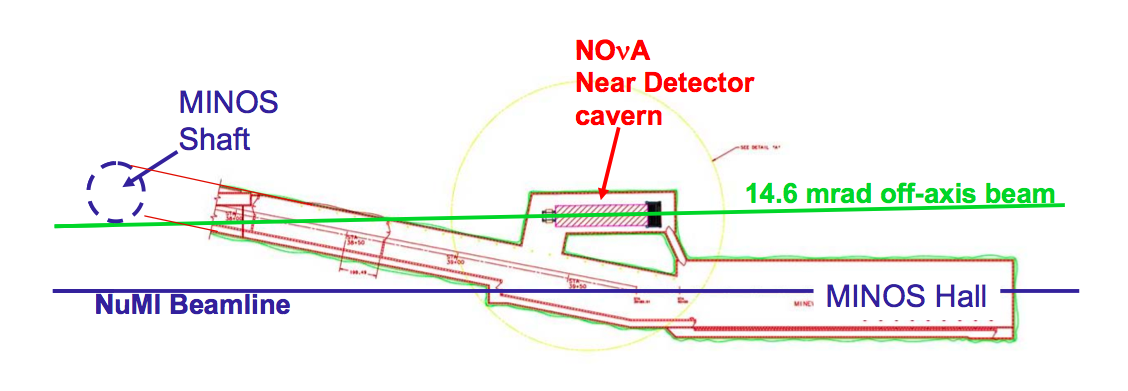
\includegraphics[width=0.8\textwidth]{../../img/baird/det/neardet_cavern_diagram.png}
  \caption{Bird's-eye view diagram of the NuMI Beam-line, MINOS Hall, MINOS
    shaft and the NOvA near detector cavern }
  \label{fig:cavern}
\end{figure}

 %near detector 
\begin{figure}
  \centering
  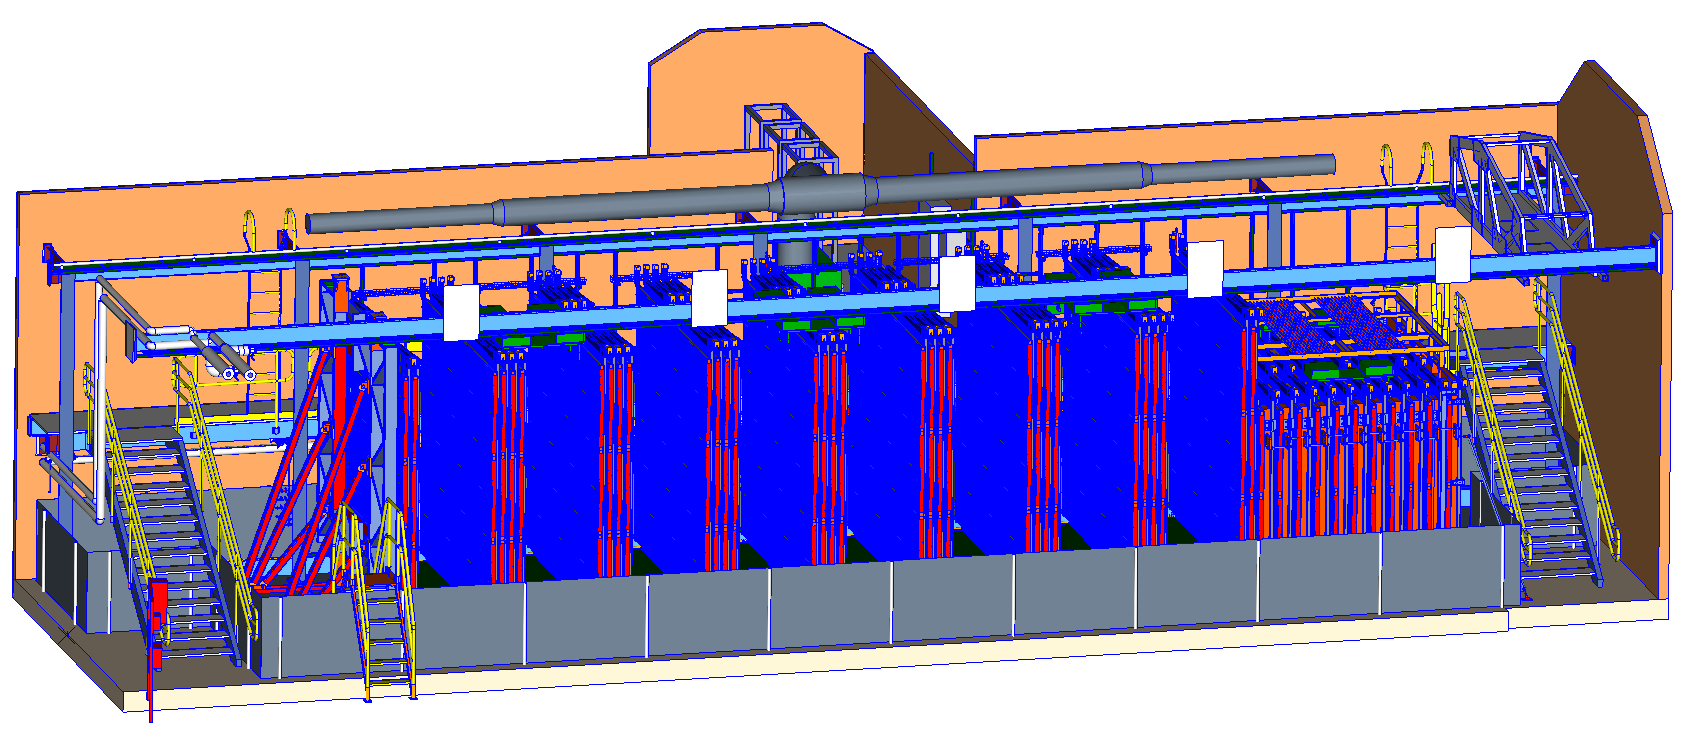
\includegraphics[width=0.8\textwidth]{../../img/baird/det/ND_01.png}
  \caption{Technical drawing of the NOvA near detector and 
    cavern. The NuMI beam enters from the left. The muon
    catcher planes are shown on the right hand side of the
    detector. Note that only some of the planes have been drawn to
    aid visualisation of the detector layout.} 
  \label{fig:neardet}
\end{figure}



\section{Monte Carlo Simulation}

%introduction
The NOvA experiment is simulated using several Monte Carlo packages.
The simulation involves several stages, each using information
from the previous step. Simulations model the
NuMI beam, subsequent neutrino interactions within the detectors,
the propagation of particles through the detector geometry, and
finally the modelling of the detector response to those particles.

% NuMI beam simulation
The creation and propapagation of the NuMI beam is simulated using FLUKA
and Geant4 through the FLUGG interface \cite{FLUKA, ferrari2005fluka,
  agostinelli2003geant4}. The beam simulation produces flux files
containing a beam of simulated neutrinos with given flavour, energy
and direction. Details of each neutrino's parent are retained in the
flux files.

% Interactions within the detector
Neutrino interactions within the detector are simulated using
GENIE \cite{andreopoulos2010genie}. 
The flux files produced by the NuMI simulation provide GENIE with a
beam of neutrinos. GENIE must decide whether each neutrino interacts
within the detector, the type of interaction, the kinematics of the
interaction and the location of the interaction vertex.
GENIE uses information regarding interaction cross sections and detector
geometry to probabilistically determine whether each neutrino
interacts within the detector. 
Figure~\ref{fig:numuCC_xsec} shows the default $\nu_\mu$ charged
current cross section as a function of neutrino energy used in GENIE.
The black data points show the results of experimental measurements,
the black curve shows the fit of theory to the data and the green
shaded band shows the estimated uncertainty. Note that there is no
data below 700~MeV.
After an initial simulated neutrino interaction the propagation of
the resulting primary particles through the nucleus, including
inter-nuclear scattering and absorption, is also simulated by
GENIE. 
%Cosmic rays
Cosmic ray generation well above the detector is simulated using CRY \cite{hagmann2007cosmic}.  

\begin{figure}
  \centering
  \includegraphics[width=0.8\textwidth]{../../img/simulation/numucc_crossSection.jpg}
  \caption{Default cross section in GENIE for $\nu_\mu$ charged
    current scattering with an isoscalar target. The shaded green band
    shows the estimated uncertainty on the free nucleon cross
    section. \cite{andreopoulos2010genie}}
  \label{fig:numuCC_xsec}
\end{figure}


%rock events


%propagation of particles through the detector
Genat4 is used to simulate the propagation and energy deposition
within the detector of the particles produced by GENIE or CRY. 
Interactions of the primary particles within the detector and the
resulting secondary particles are also simulated.
The resulting energy depositions within the detectors liquid
scintillator are recorded and are known as Fibre Liquid Scintillator
Hist (FLSHits). 

%readout response
Next two NOvA specific software modules are used to simulate the
response of the NOvA detectors to energy depositions
\cite{adamNOvASim, adamNOvASimProceedings}. 
The first module simulates the processes from FLSHit in a NOvA cell to photons
arriving at the APD. The final APD signal is a combination of the
photons arriving at the APD and the APDs modelled response to noise.
The second module simulates the response of the FEBs to the APD
signals.  